\documentclass[12pt]{article}
\usepackage[spanish, english, es-tabla]{babel}
\usepackage[utf8]{inputenc}
\usepackage[left = 2cm, right = 2cm, bottom = 2cm, top = 3cm]{geometry}
\usepackage{amsmath, amssymb}
\usepackage{graphicx}
\usepackage{hyperref}
\usepackage{listings}
\usepackage{courier}

\usepackage[dvipsnames]{xcolor}

\renewcommand{\lstlistingname}{Código}
\renewcommand{\lstlistlistingname}{Listado de códigos}

% https://tex.stackexchange.com/questions/60209/how-to-add-an-extra-level-of-sections-with-headings-below-subsubsection
\newcommand{\subsubsubsection}[1]{\paragraph{#1}\mbox{}\\}
\setcounter{secnumdepth}{4}
\setcounter{tocdepth}{4}

% Configure lstlisting
\definecolor{codegreen}{rgb}{0,0.6,0}
\definecolor{codegray}{rgb}{0.5,0.5,0.5}
\definecolor{codepurple}{rgb}{0.58,0,0.82}
\definecolor{backcolour}{rgb}{0.95,0.95,0.92}

\lstdefinestyle{mystyle}{
	backgroundcolor=\color{backcolour},   
	commentstyle=\color{codegreen},
	keywordstyle=\color{magenta},
	numberstyle=\tiny\color{codegray},
	stringstyle=\color{codepurple},
	basicstyle=\ttfamily\footnotesize,
	breakatwhitespace=false,         
	breaklines=true,                 
	captionpos=t,                    
	keepspaces=true,                 
	numbers=left,                    
	numbersep=5pt,                  
	showspaces=false,                
	showstringspaces=false,
	showtabs=false,                  
	tabsize=2
}

\lstset{style=mystyle}


\begin{document}
	\selectlanguage{spanish}
	
	\title{Proyecto 2. Procesado de imágenes usando morfología matemática con \texttt{MATLAB} \\ \textit{\textbf{\large Máster Universitario en Ingeniería de Telecomunicación}} \\ \textit{\large Procesado de señales acústicas e imágenes}}
	\author{Enrique Fernández Sánchez \\ Link al código: \href{https://github.com/Raniita/image-processing-matlab/tree/main/morfologia}{Github: Raniita/image-processing-matlab}}
	
	\maketitle
	
	\vspace{120px}
	
	\tableofcontents
	
	\pagebreak
	
	%\addcontentsline{toc}{section}{Listado de códigos}
	\lstlistoflistings
	
	\listoffigures
	
	\pagebreak
	
	\section{Detectar placas de calles}
	
	\noindent En este apartado vamos a comentar la implementación de mi ``script'' para detectar placas de calles, utilizando morfología matemática con \texttt{MATLAB}. \\
	
	\noindent El código completo de mi implementación lo encontramos en la sección: \ref{section: codigo}.
	
	\subsection{Primera implementación}
	\noindent A modo de ejemplo, voy a ir comentando cada uno de los pasos que sigue una imagen hasta llegar a su segmentación final y posterior procesado del OCR.
	
	\begin{enumerate}
		\item \textbf{Lectura de la imagen}.
		\begin{lstlisting}[language=matlab, caption={Lectura de la imagen}]
% Leer imagen
img = imread(['./photos/' dataset_images{j}]);
img_rgb = img;
img = im2double(rgb2gray(img));
%figure, imagesc(img), axis off image, colormap gray
		\end{lstlisting}
	
		\begin{figure}[h!]
			\begin{center}
				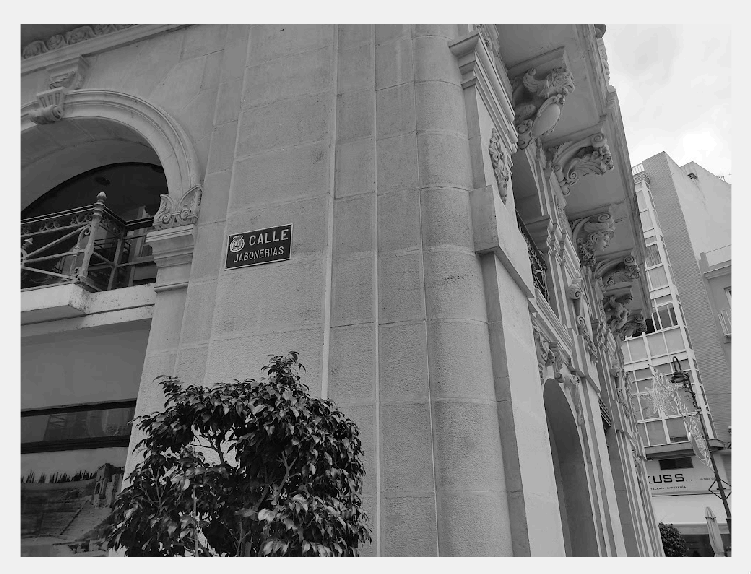
\includegraphics[width=0.75\textwidth]{img/impl_1.png}
				\caption{Lectura de la imagen}
				\label{img: lectura}
			\end{center}
		\end{figure}
	
		\pagebreak
	
		\item \textbf{Detectar bordes}. En este primer ejemplo de implementación, he utilizado una función para detectar bordes que no es morfologíca. Dicha función es \texttt{edge}, que busca los bordes de la imagen en función de la intensidad de esta. Para ello, ajustamos el valor de \texttt{threshold} en el que se detectan los bordes.
		\begin{lstlisting}[language=matlab, caption={Detectar bordes I}]
% Detectar bordes (segmentacion)
[x, thresshold] = edge(img, 'sobel');
% Valor de ajuste para resaltar todavia mas los bordes de la placa
k = 1.2;  
mask = edge(img, 'sobel', thresshold * k);
%figure, imagesc(mask), axis off image, colormap gray
		\end{lstlisting}
	
		\begin{figure}[h!]
			\begin{center}
				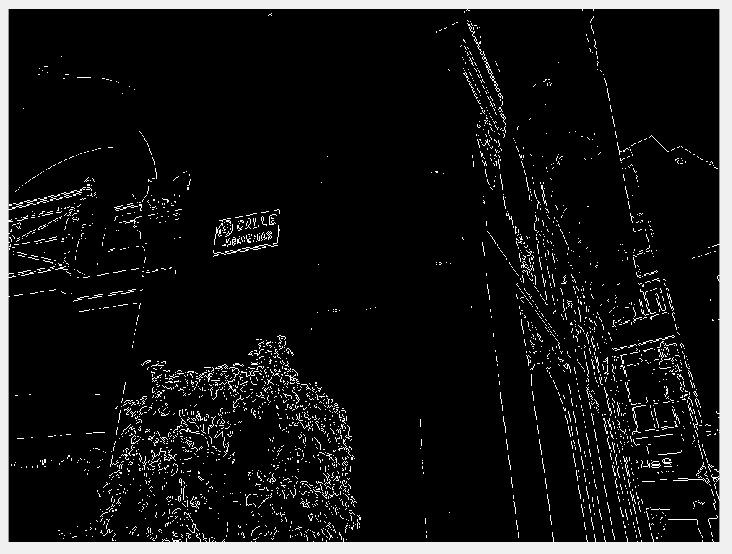
\includegraphics[width=0.85\textwidth]{img/impl_2.png}
				\caption{Detección de bordes I}
				\label{img: bordes 1}
			\end{center}
		\end{figure}
	
		\pagebreak
		
		\item \textbf{Dilatar imagen}. En este paso procedemos a dilatar la imagen con dos elementos estructurantes, estos elementos son dos lineas del mismo tamaño, situadas cada una a 0 y 90 grados respectivamente. Con esto conseguimos dilatar todavía más los bordes de la calle, además de detectar todas esas formas que tienen más pinta de linea recta en sus bordes.
		\begin{lstlisting}[language=matlab, caption={Dilatar la imagen}]
% Dilatar la imagen
struct_elem90 = strel('line', 12, 90);
struct_elem0 = strel('line', 12, 0);
mask_dilate = imdilate(mask, [struct_elem90 struct_elem0]);
%figure, imagesc(mask_dilate), axis off image, colormap gray
		\end{lstlisting}
	
		\begin{figure}[h!]
			\begin{center}
				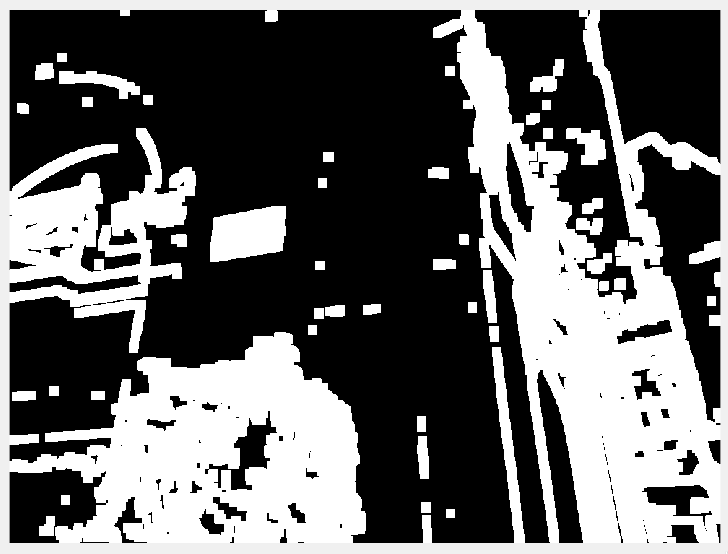
\includegraphics[width=0.85\textwidth]{img/impl_3.png}
				\caption{Dilatar la imagen}
				\label{img: dilatar imagen}
			\end{center}
		\end{figure}
	
		\pagebreak
		
		\item \textbf{Llenar brechas interiores}. En este paso pretendo rellenar todos los posibles huecos que puedan encontrarse dentro de una región que ya ha sido dilatada. En principio con el paso anterior ya debería estar suficiente relleno, sin embargo nos vendrá bien aplicar este paso ya que nos mejora los resultados del paso siguiente.
		\begin{lstlisting}[language=matlab, caption={Llenar brechas interiores}]
% Llenar brechas interiores
mask_fill = imfill(mask_dilate, 'holes');
%figure, imagesc(mask_fill), axis off image, colormap gray
		\end{lstlisting}
	
		\begin{figure}[h!]
			\begin{center}
				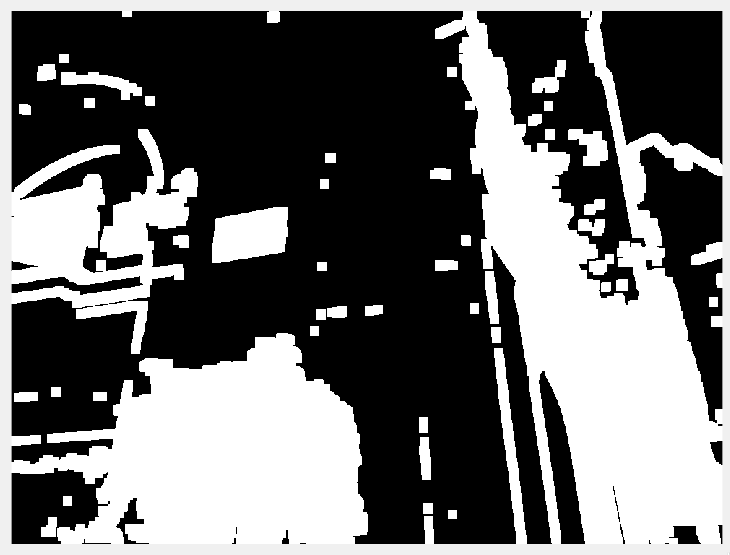
\includegraphics[width=0.85\textwidth]{img/impl_4.png}
				\caption{Llenar brechas interiores}
				\label{img: brechas interiores}
			\end{center}
		\end{figure}
	
		\pagebreak
		
		\item \textbf{Retirar los bordes no conectados con el borde}. Este paso nos permite eliminar todas las estructuras de la imagen que no están conectadas con el borde de la imagen. Esto nos limpia mucho la imagen, dejando prácticamente la placa de la calle ya segmentada. El valor 4 hace referencia a que los pixeles conectados son aquellos en los que los bordes se tocan, también podemos sustituir por 8, que hace referencia a que los bordes o esquinas se tocan.
		\begin{lstlisting}[language=matlab, caption={Retirar los objetos no conectados con el borde}]
% Retirar los objetos no conectados con el borde
mask_noborder = imclearborder(mask_fill, 4);
%figure, imagesc(mask_noborder), axis off image, colormap gray,
		\end{lstlisting}
	
		\begin{figure}[h!]
			\begin{center}
				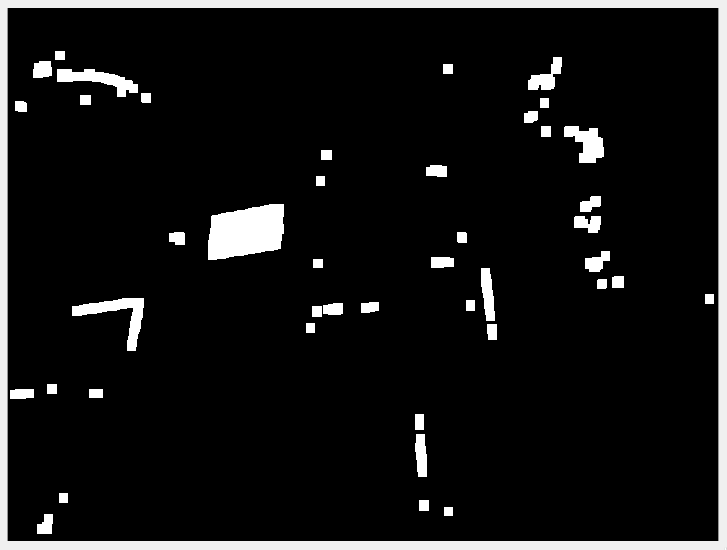
\includegraphics[width=0.85\textwidth]{img/impl_5.png}
				\caption{Retirar objetos no conectados con el borde}
				\label{img: objetos no conectados}
			\end{center}
		\end{figure}
	
		\pagebreak
		
		\item \textbf{Suavizado del objeto}. Con el objetivo de eliminar todos esos elementos residuales que quedan en la imagen, aplicamos un suavizado con un elemento estructurante de dimensiones similares a las de la placa a segmentar.
		\begin{lstlisting}[language=matlab, caption={Suavizamos el objeto con elemento estructurante rectangular}]
% Suavizamos el objeto
struct_elemD = strel('rectangle', [12 15]);
mask_final = imerode(mask_noborder, struct_elemD);
mask_final = imerode(mask_final, struct_elemD);
%figure, imagesc(mask_final), axis off image, colormap gray
		\end{lstlisting}
	
		\begin{figure}[h!]
			\begin{center}
				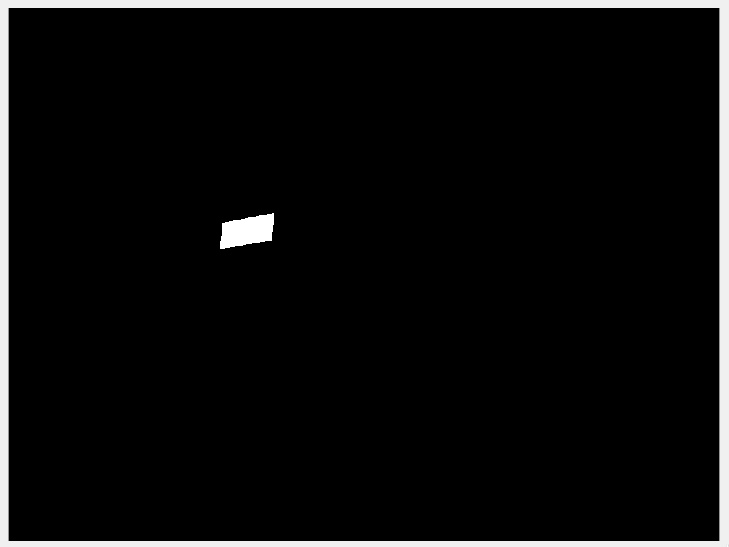
\includegraphics[width=0.85\textwidth]{img/impl_6.png}
				\caption{Suavizamos el objeto con elemento estructurante rectangular}
				\label{img: suavizado}
			\end{center}
		\end{figure}
	
		\pagebreak
		
		\item \textbf{Multiplicación con imagen inicial}. En este paso, ya tenemos una máscara binaria con la posición de la placa de la calle, por lo que tendremos que multiplicarlo con la imagen inicial. Además, aplicamos un pequeño filtrado morfológico para aumentar el detalle de las letras de la placa, con el objetivo de facilitar al OCR la detección de los caracteres.
		\begin{lstlisting}[language=matlab, caption={Multiplicación con imagen inicial}]
% Multiplicar
img_mult = immultiply(img, mask_final);
se_close = strel('line', 3, 90);
img_mult = imclose(img_mult, se_close);
%figure, imagesc(img_mult), axis off image, colormap gray
		\end{lstlisting}
	
		\begin{figure}[h!]
			\begin{center}
				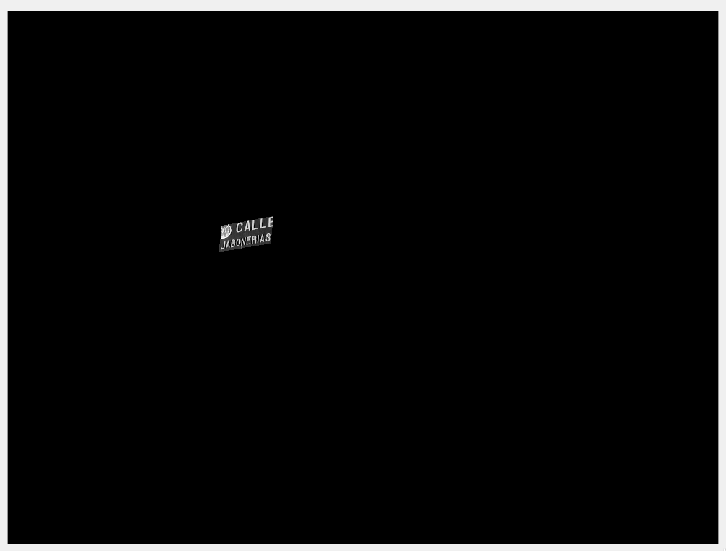
\includegraphics[width=0.85\textwidth]{img/impl_7.png}
				\caption{Multiplicación con imagen inicial}
				\label{img: multiplicacion}
			\end{center}
		\end{figure}
	
		\pagebreak
		
		\item Aplicar OCR e imagen final. En este último paso, aplicamos OCR sobre la imagen obtenida en el paso anterior. Para ello, he tenido que descargar un dataset de \textit{tesseract} entrenado para el lenguaje español. La información obtenida por el OCR se ha representado en la figura, además del grado de confianza de la predicción. 
		\begin{lstlisting}[language=matlab, caption={Aplicar OCR e imagen final}]
% OCR
% SRC: https://es.mathworks.com/help/vision/ref/ocr.html
% SRC: https://es.mathworks.com/help/vision/ug/recognize-text-using-optical-character-recognition-ocr.html
% SRC traineddata: https://github.com/tesseract-ocr/tessdata/blob/074c37215b01ab8cc47a0e06ff7356383883d775/spa.traineddata
results_ocr = ocr(img_mult, 'TextLayout', 'Block', 'Language', {'./tessdata/spa_old_2015.traineddata'});
%results_ocr = ocr(img_mult, 'TextLayout', 'Block');

% Obtenemos el texto del OCR
string_calle = '';
for i=1:length(results_ocr.Words)
	if i==1
		string_calle = results_ocr.Words{i};
	else
		string_calle = strcat(string_calle, [' ' results_ocr.Words{i}]);
	end
end
disp(['El nombre de la calle es: ' string_calle])

% Grado de confianza
grade_confidence = mean(results_ocr.WordConfidences);
str_confidence = ['Media confianza: ' num2str(grade_confidence)];
disp(str_confidence);

% Overlay
% SRC: https://es.mathworks.com/help/vision/ref/ocr.html
figure('Position', get(0, 'Screensize')),
imagesc(imfuse(img_rgb, mask_final, 'blend')),
axis off image,
colormap gray,
title(['Detectar calle en imagen: ' strrep(dataset_images{j},'_',' ')])
% Nombre de la calle
text(10, 20, string_calle, 'BackgroundColor', [1 1 1])
% Confianza
text(10, 60, str_confidence, 'BackgroundColor', [1 1 1])
		\end{lstlisting}
	
	\pagebreak
	
	\noindent Tal y como podemos ver en la figura siguiente, la predicción del OCR no es 100\% exacta para esta imagen, ya que depende de muchos factores. Se podrían aplicar técnicas para mejorar las letras del interior de la placa y ver si el resultado obtenido mejora. Sin embargo, dada la diferencia entre las diferentes fotos escogidas para el trabajo, se hacia realmente difícil que todas las imagen arrojaran una buena predicción en el OCR.
	
		\begin{figure}[h!]
			\begin{center}
				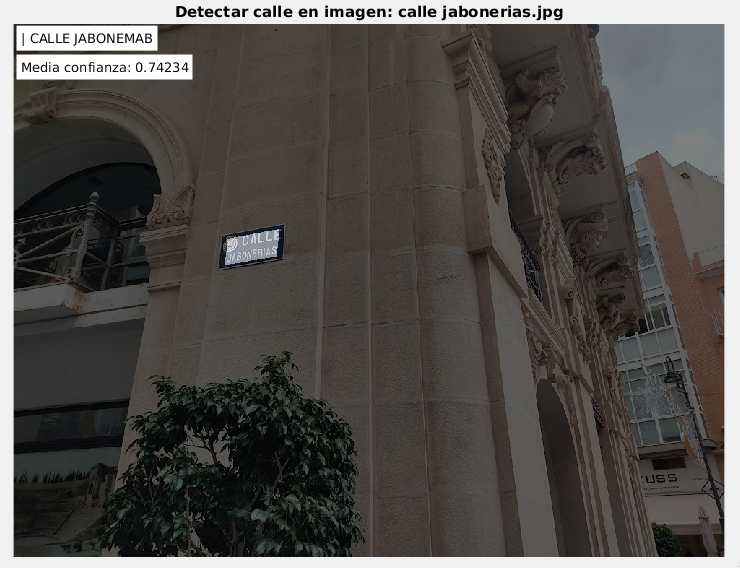
\includegraphics[width=1\textwidth]{img/impl_8.png}
				\caption{Aplicar OCR e imagen final}
				\label{img: ocr}
			\end{center}
		\end{figure}
	
	\end{enumerate}

	\pagebreak

	\subsection{Segunda implementación}
	\noindent Por otro lado, he sustituido la detección de bordes de la implementación anterior con un método de gradiente morfológico, con el objetivo de maximizar los métodos vistos en esta parte de la asignatura. Para ello, vamos a comentar los resultados de la misma imagen utilizada en el apartado anterior. \\
	
	\noindent Procedo a repasar los pasos de la implementación anterior, pero aplicando el cambio mencionado.
	
	\begin{enumerate}
		\item \textbf{Lectura de la imagen}. Equivalente al apartado anterior. \\
		
		\item \textbf{Detectar bordes usando morfología}. Para esta implementación hemos obtenido el gradiente morfológico, y posteriormente transformado la salida a una imagen binarizada, con el objetivo de equiparar ambas implementaciones.
		
		\begin{lstlisting}[language=matlab, caption={Deteccion de bordes II}]
% Detecctar bordes (gradiente morfologico)
% SRC: https://blogs.mathworks.com/steve/2006/09/25/dilation-erosion-and-the-morphological-gradient/
struc_elemGrad = strel('diamond', 2);
mask = im2bw(imdilate(img, struc_elemGrad) - imerode(img, struc_elemGrad));
%figure, imagesc(mask), axis off image, colormap gray, colorbar
		\end{lstlisting}
	
		\begin{figure}[h!]
			\begin{center}
				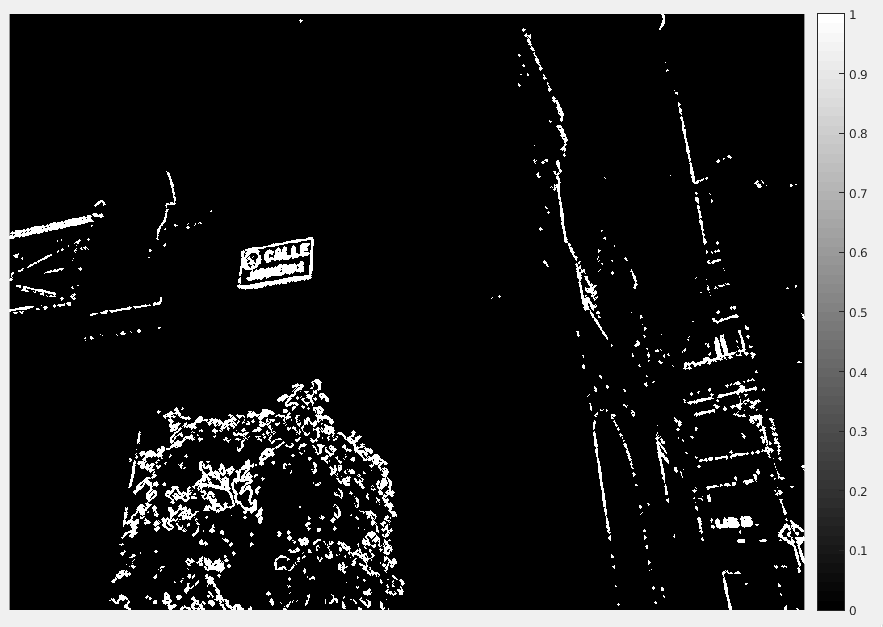
\includegraphics[width=0.8\textwidth]{img/impl_9.png}
				\caption{Detección de bordes II}
				\label{img: bordes II}
			\end{center}
		\end{figure}
	
		\pagebreak
		
		\item \textbf{Dilatar imagen}.
		
		\begin{figure}[h!]
			\begin{center}
				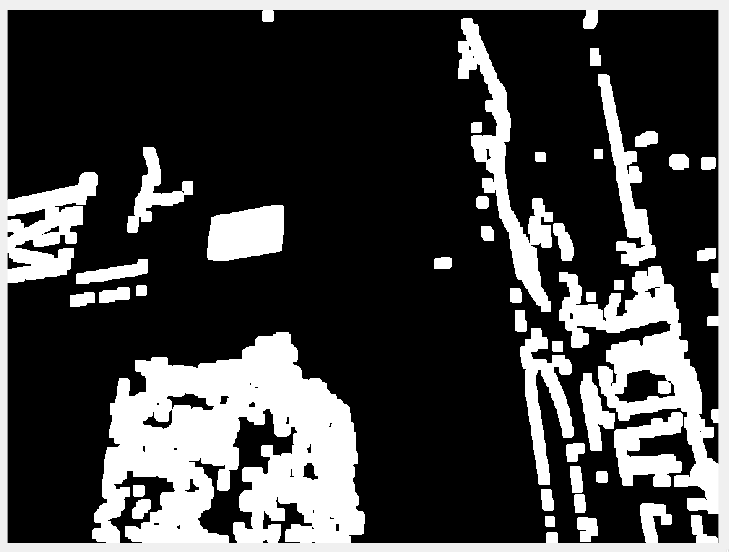
\includegraphics[width=0.65\textwidth]{img/impl_10.png}
				\caption{Dilatar imagen}
				\label{img: dilatar 2}
			\end{center}
		\end{figure}
		
		\item \textbf{Llenar brechas interiores}.
		
		\begin{figure}[h!]
			\begin{center}
				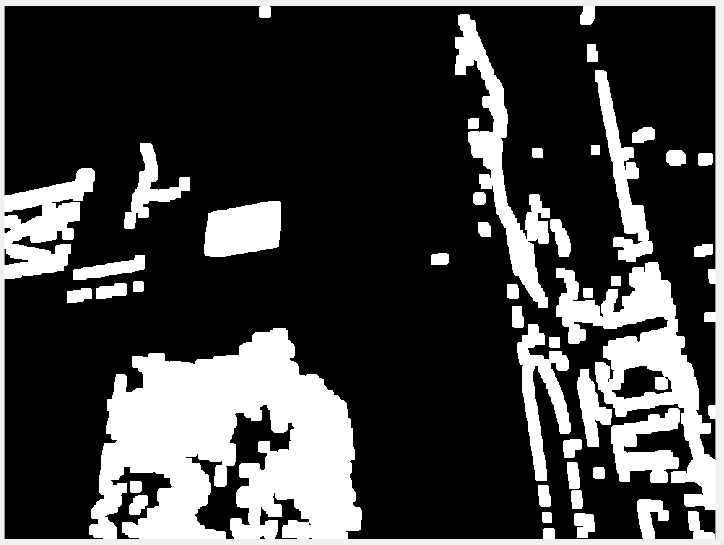
\includegraphics[width=0.65\textwidth]{img/impl_11.png}
				\caption{Llenar brechas interiores}
				\label{img: brechas 2}
			\end{center}
		\end{figure}
	
		\pagebreak
		
		\item \textbf{Retirar los objetos no conectados con el borde}.
		
		\begin{figure}[h!]
			\begin{center}
				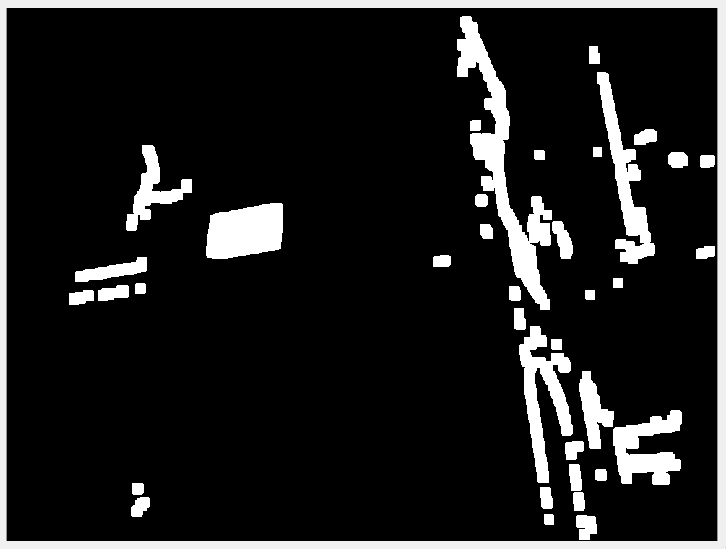
\includegraphics[width=0.65\textwidth]{img/impl_12.png}
				\caption{Retirar objetos no conectados con el borde}
				\label{img: retirar obj 2}
			\end{center}
		\end{figure}
		
		\item \textbf{Suavizado del objeto}.
		
		\begin{figure}[h!]
			\begin{center}
				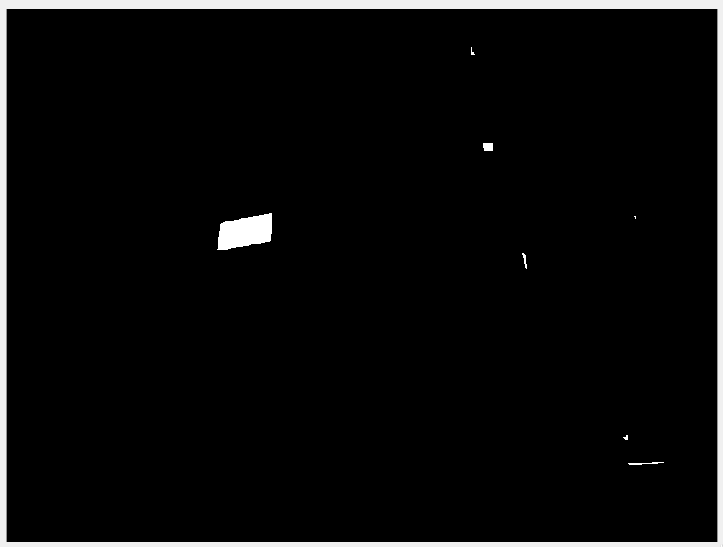
\includegraphics[width=0.65\textwidth]{img/impl_13.png}
				\caption{Suavizado del objeto}
				\label{img: suavizado 2}
			\end{center}
		\end{figure}
	
		\pagebreak
		
		\item \textbf{Multiplicación con imagen inicial}.
		
		\begin{figure}[h!]
			\begin{center}
				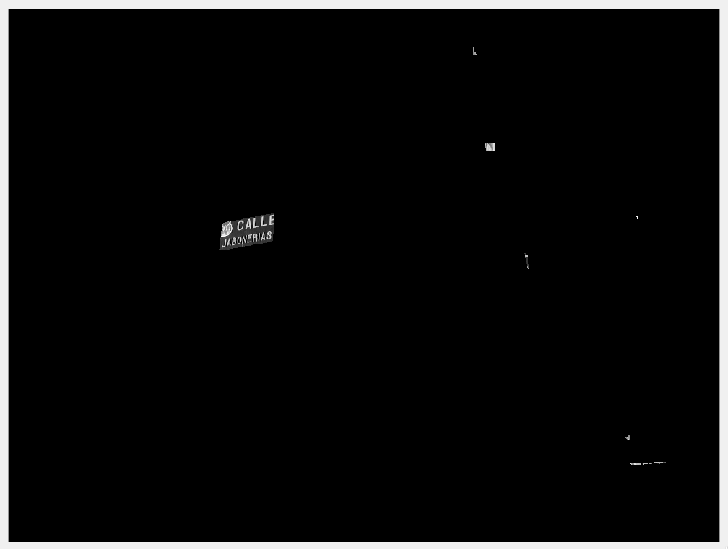
\includegraphics[width=0.65\textwidth]{img/impl_14.png}
				\caption{Multiplicación con imagen inicial}
				\label{img: mult 2}
			\end{center}
		\end{figure}
		
		\item \textbf{Aplicar OCR e imagen final}.
		
		\begin{figure}[h!]
			\begin{center}
				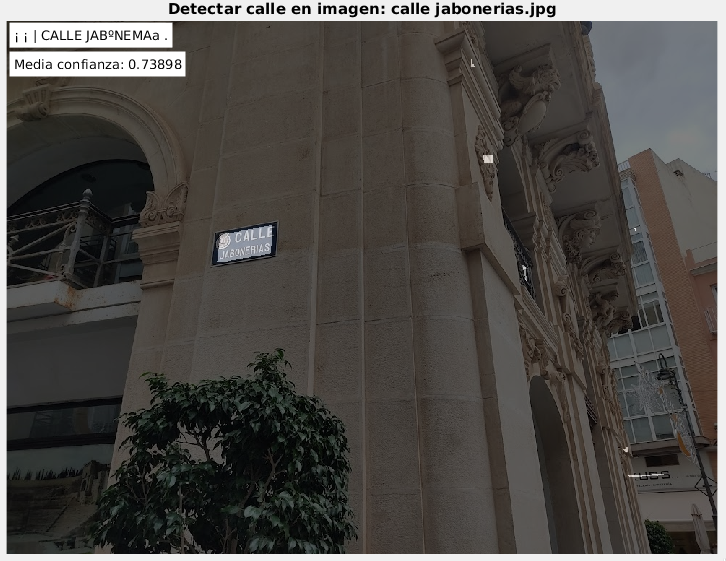
\includegraphics[width=0.65\textwidth]{img/impl_15.png}
				\caption{Aplicar OCR e imagen final}
				\label{img: final 2}
			\end{center}
		\end{figure}
	\end{enumerate}

	\subsection{Diez imágenes de la primera implementación}
		\begin{figure}[h!]
			\begin{center}
				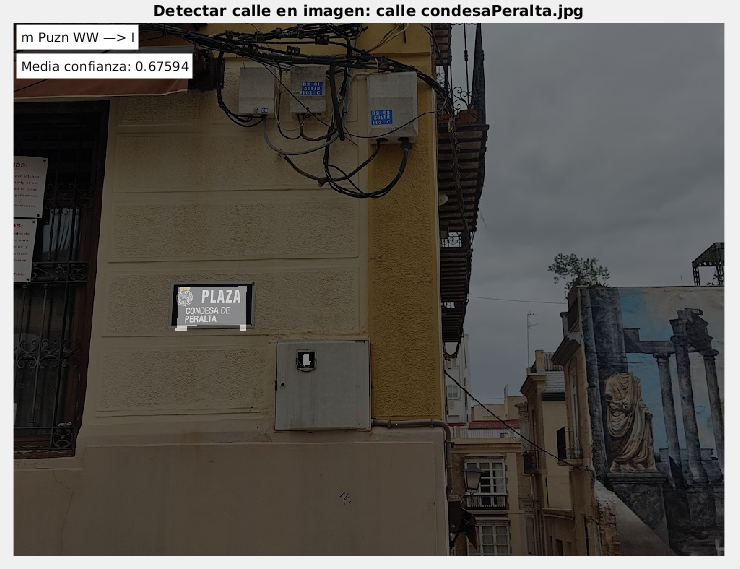
\includegraphics[width=0.65\textwidth]{img/1_1.png}
				\caption{[1] Imagen final Plaza Condesa de Peralta}
			\end{center}
		\end{figure}
	
		\begin{figure}[h!]
			\begin{center}
				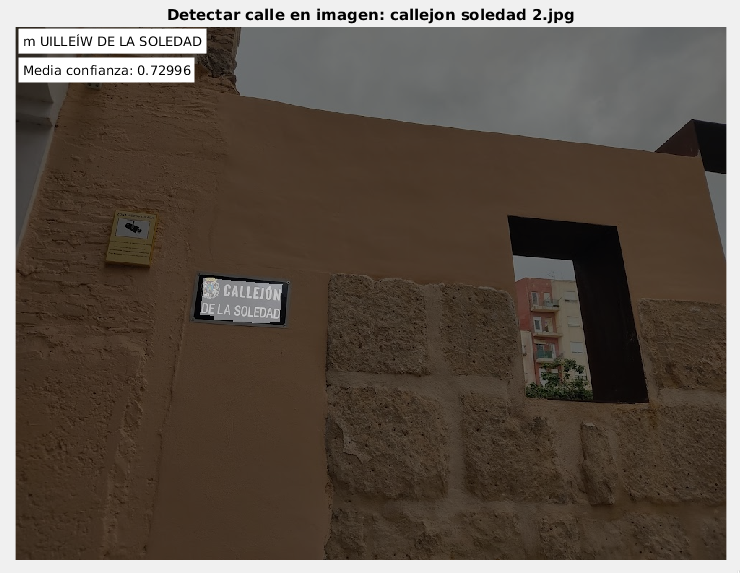
\includegraphics[width=0.65\textwidth]{img/1_2.png}
				\caption{[1] Imagen final Callejón de la Soledad}
			\end{center}
		\end{figure}
	
		\pagebreak
		
		\begin{figure}[h!]
			\begin{center}
				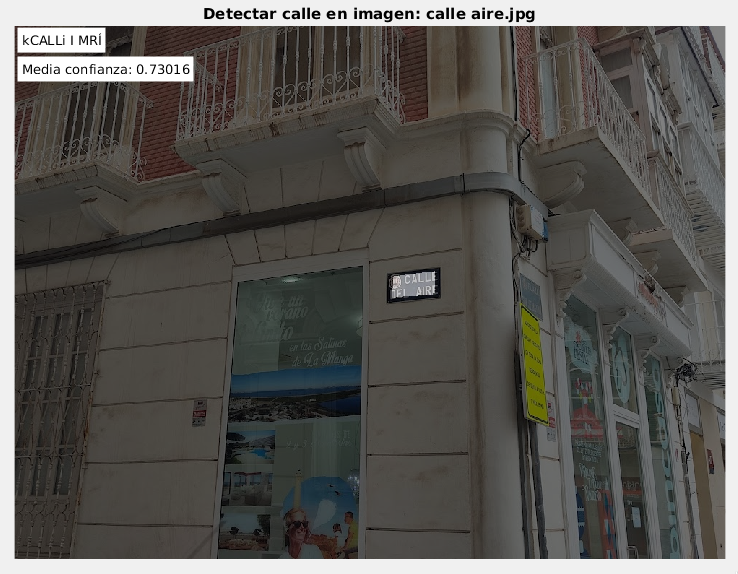
\includegraphics[width=0.65\textwidth]{img/1_3.png}
				\caption{[1] Imagen final Calle del Aire}
			\end{center}
		\end{figure}
		
		\begin{figure}[h!]
			\begin{center}
				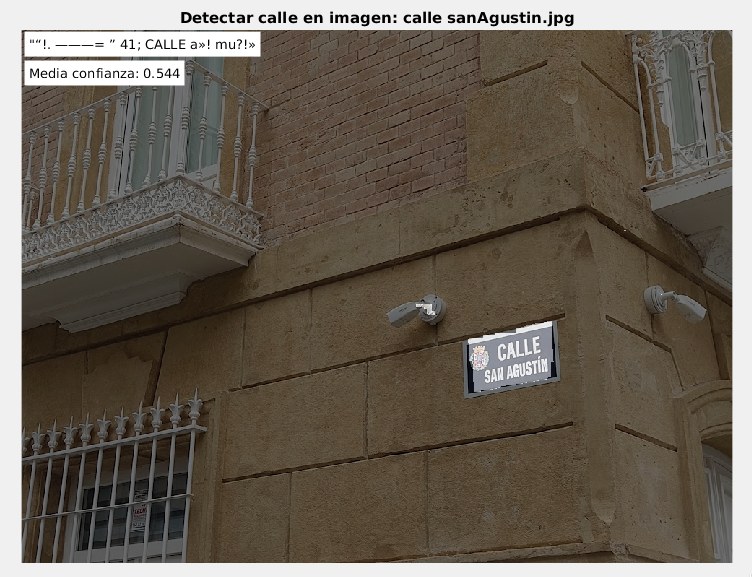
\includegraphics[width=0.65\textwidth]{img/1_4.png}
				\caption{[1] Imagen final Calle San Agustín}
			\end{center}
		\end{figure}
		
		\pagebreak
		
		\begin{figure}[h!]
			\begin{center}
				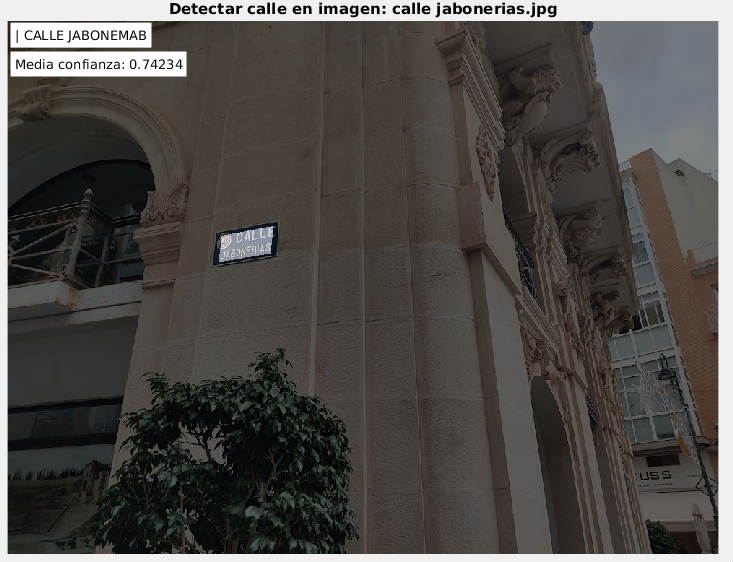
\includegraphics[width=0.65\textwidth]{img/1_5.png}
				\caption{[1] Imagen final Calle Jabonerías}
			\end{center}
		\end{figure}
		
		\begin{figure}[h!]
			\begin{center}
				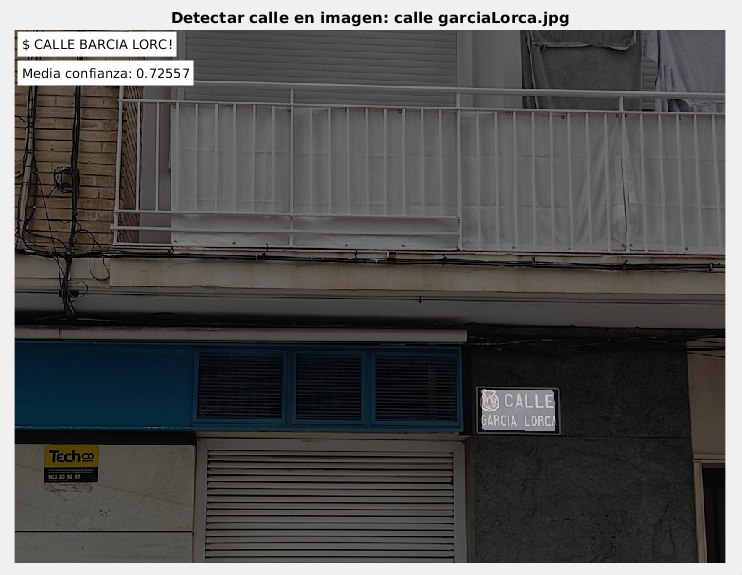
\includegraphics[width=0.65\textwidth]{img/1_6.png}
				\caption{[1] Imagen final Calle Garcia Lorca}
			\end{center}
		\end{figure}
		
		\pagebreak
		
		\begin{figure}[h!]
			\begin{center}
				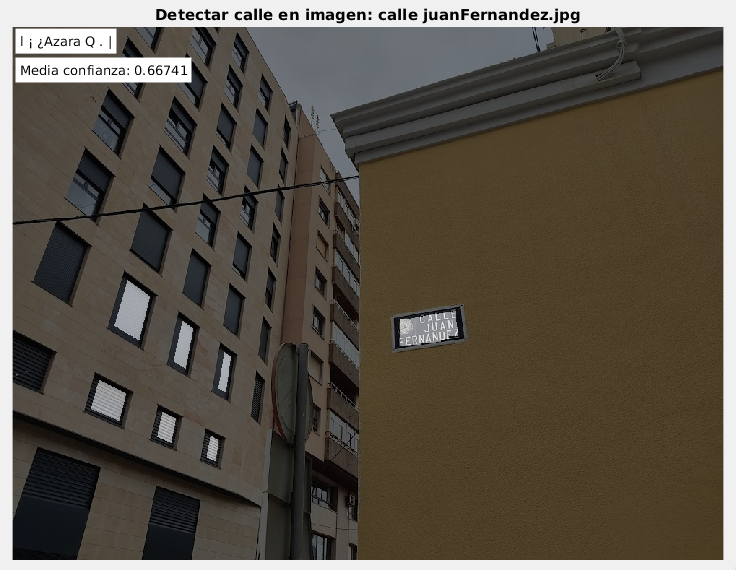
\includegraphics[width=0.65\textwidth]{img/1_7.png}
				\caption{[1] Imagen final Calle Juan Fernández}
			\end{center}
		\end{figure}
		
		\begin{figure}[h!]
			\begin{center}
				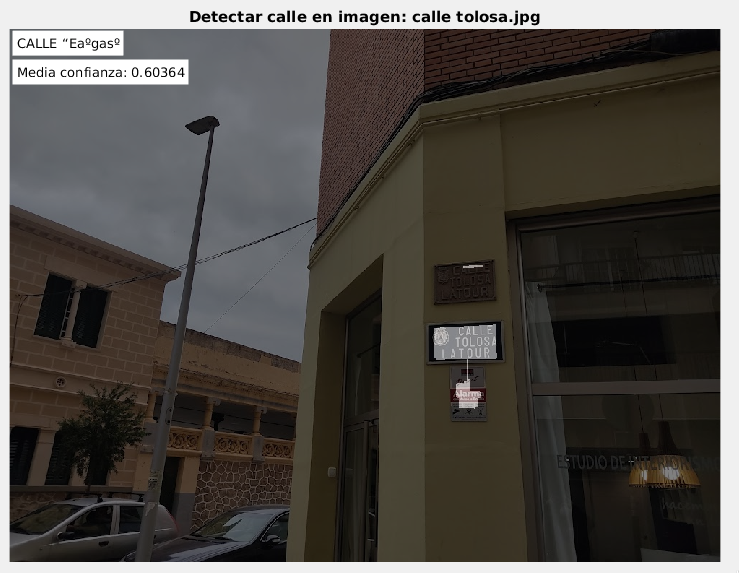
\includegraphics[width=0.65\textwidth]{img/1_8.png}
				\caption{[1] Imagen final Calle Tolosa La Tour}
			\end{center}
		\end{figure}
		
		\pagebreak
		
		\begin{figure}[h!]
			\begin{center}
				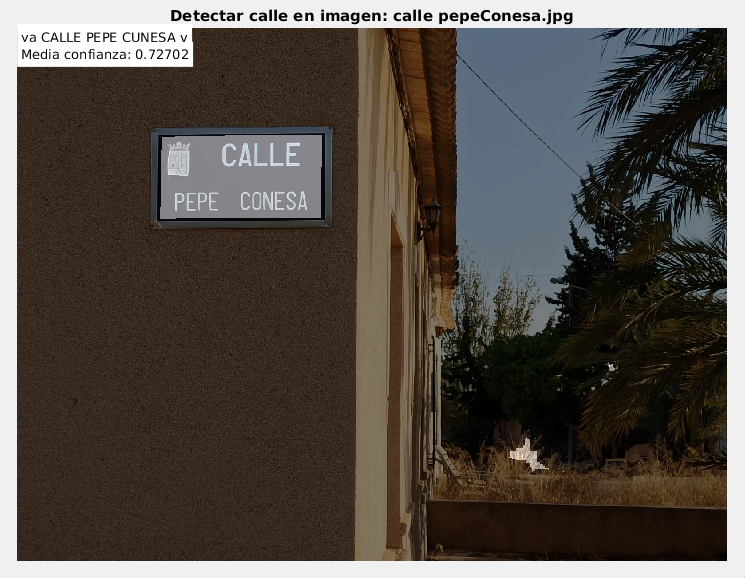
\includegraphics[width=0.65\textwidth]{img/1_9.png}
				\caption{[1] Imagen final Calle Pepe Conesa}
			\end{center}
		\end{figure}
		
		\begin{figure}[h!]
			\begin{center}
				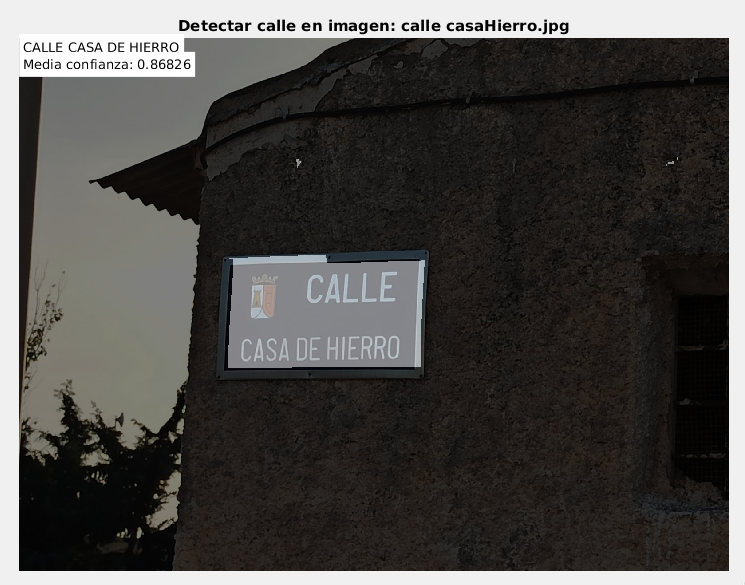
\includegraphics[width=0.65\textwidth]{img/1_10.png}
				\caption{[1] Imagen final Calle Casa de Hierro}
			\end{center}
		\end{figure}
	
	\pagebreak
	
	\subsection{Diez imágenes de la segunda implementación}
	\noindent En esta implementación hay algunas imágenes que no conseguimos encontrar el cartel de las calles, sin embargo, las he dejado ya que he considerado que sería bastante ilustrativo la diferencia entre ambas implementaciones, además de las diferencias ya existentes en los resultados obtenidos por el OCR.
	
	\begin{figure}[h!]
		\begin{center}
			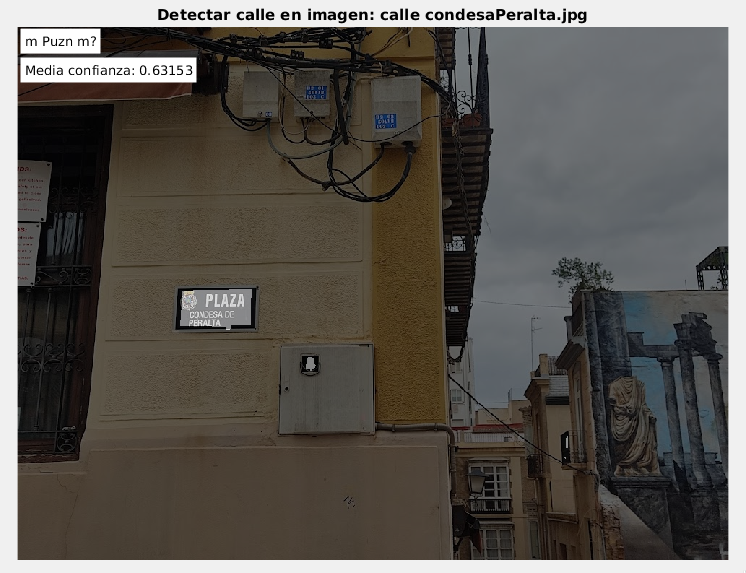
\includegraphics[width=0.55\textwidth]{img/2_1.png}
			\caption{[2] Imagen final Plaza Condesa de Peralta}
		\end{center}
	\end{figure}
	
	\begin{figure}[h!]
		\begin{center}
			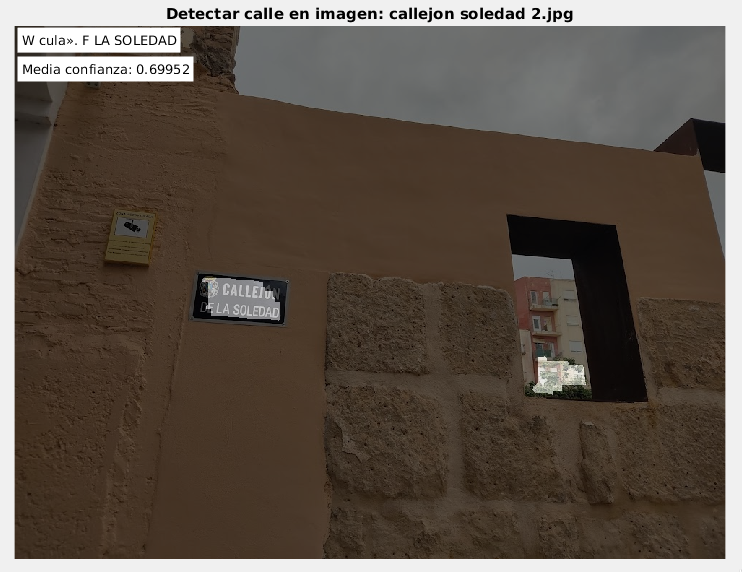
\includegraphics[width=0.55\textwidth]{img/2_2.png}
			\caption{[2] Imagen final Callejón de la Soledad}
		\end{center}
	\end{figure}
	
	\pagebreak
	
	\begin{figure}[h!]
		\begin{center}
			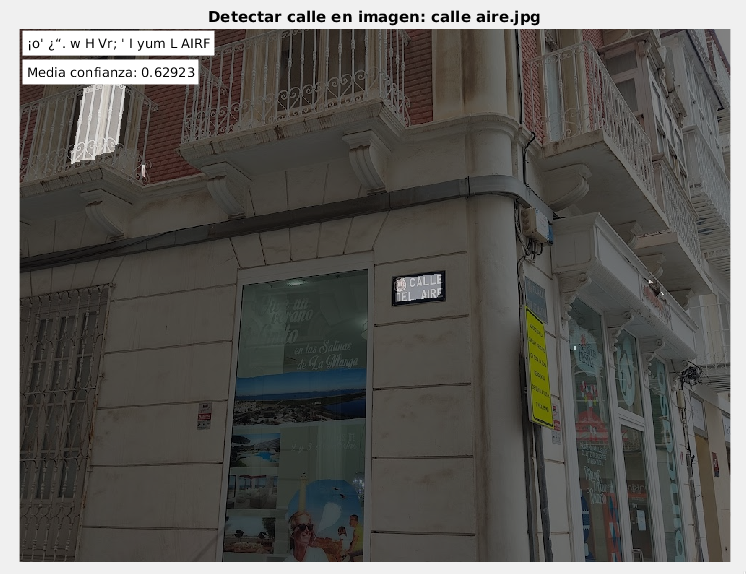
\includegraphics[width=0.65\textwidth]{img/2_3.png}
			\caption{[2] Imagen final Calle del Aire}
		\end{center}
	\end{figure}
	
	\begin{figure}[h!]
		\begin{center}
			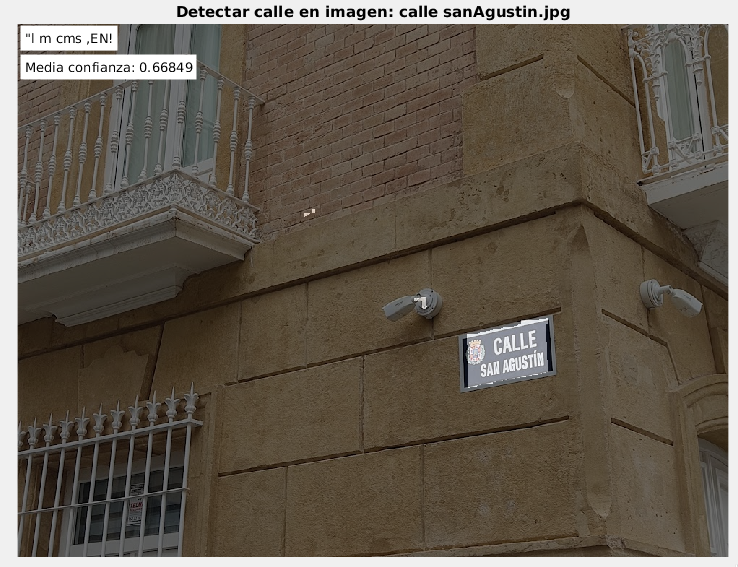
\includegraphics[width=0.65\textwidth]{img/2_4.png}
			\caption{[2] Imagen final Calle San Agustín}
		\end{center}
	\end{figure}
	
	\pagebreak
	
	\begin{figure}[h!]
		\begin{center}
			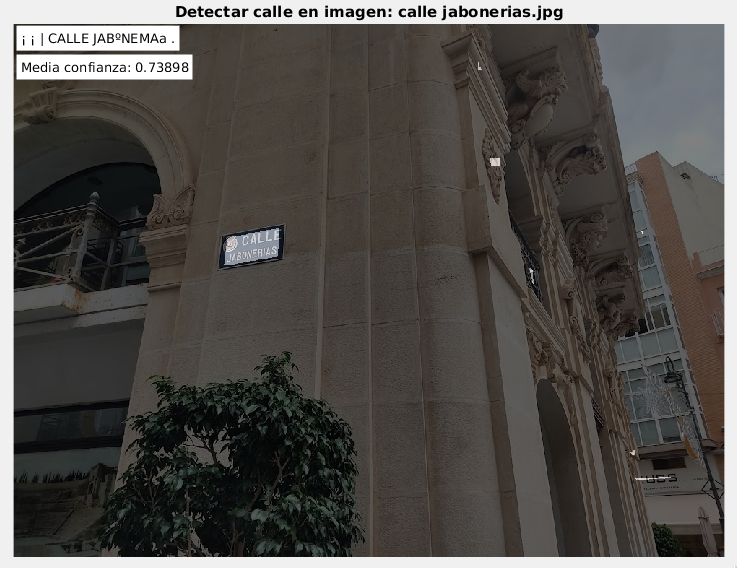
\includegraphics[width=0.65\textwidth]{img/2_5.png}
			\caption{[2] Imagen final Calle Jabonerías}
		\end{center}
	\end{figure}
	
	\begin{figure}[h!]
		\begin{center}
			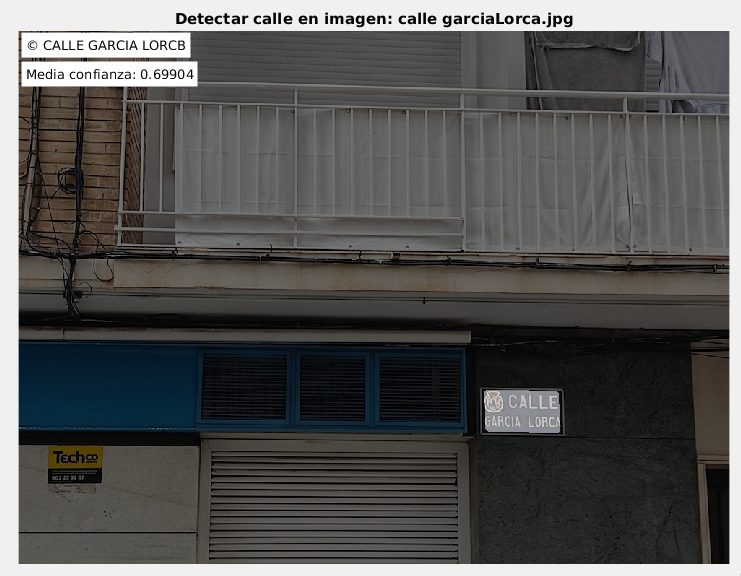
\includegraphics[width=0.65\textwidth]{img/2_6.png}
			\caption{[2] Imagen final Calle Garcia Lorca}
		\end{center}
	\end{figure}
	
	\pagebreak
	
	\begin{figure}[h!]
		\begin{center}
			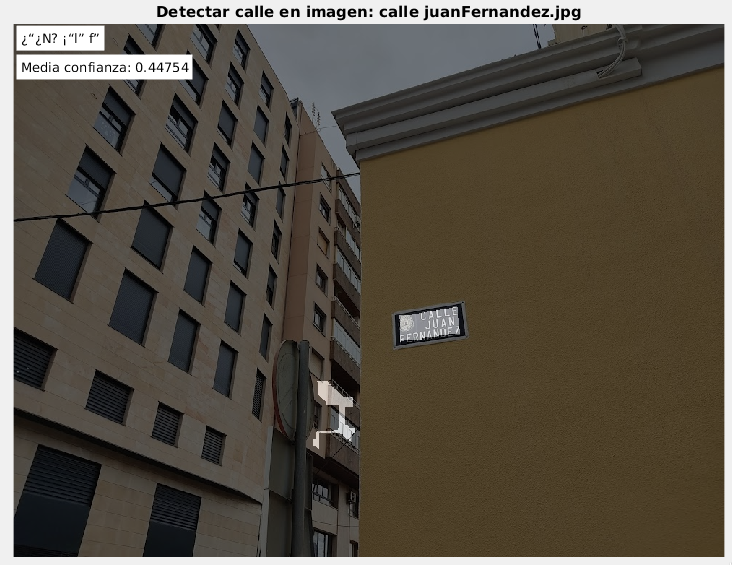
\includegraphics[width=0.65\textwidth]{img/2_7.png}
			\caption{[2] Imagen final Calle Juan Fernández}
		\end{center}
	\end{figure}
	
	\begin{figure}[h!]
		\begin{center}
			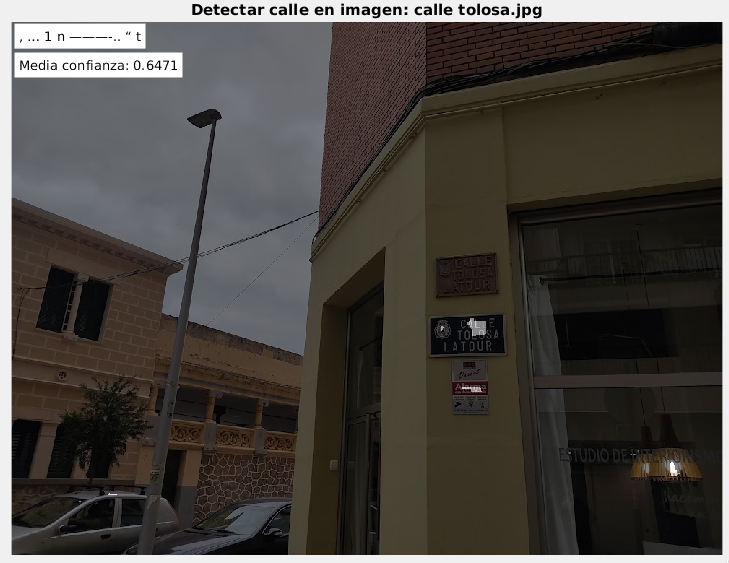
\includegraphics[width=0.65\textwidth]{img/2_8.png}
			\caption{[2] Imagen final Calle Tolosa la Tour}
		\end{center}
	\end{figure}
	
	\pagebreak
	
	\begin{figure}[h!]
		\begin{center}
			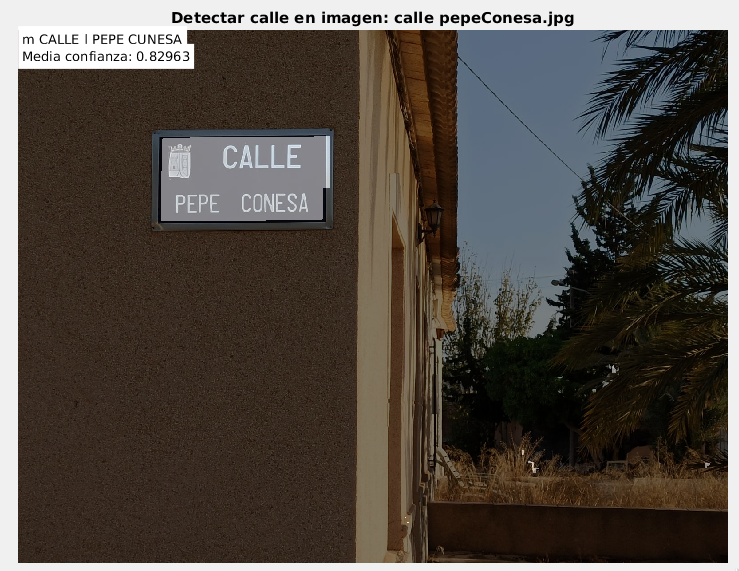
\includegraphics[width=0.65\textwidth]{img/2_9.png}
			\caption{[2] Imagen final Calle Pepe Conesa}
		\end{center}
	\end{figure}
	
	\begin{figure}[h!]
		\begin{center}
			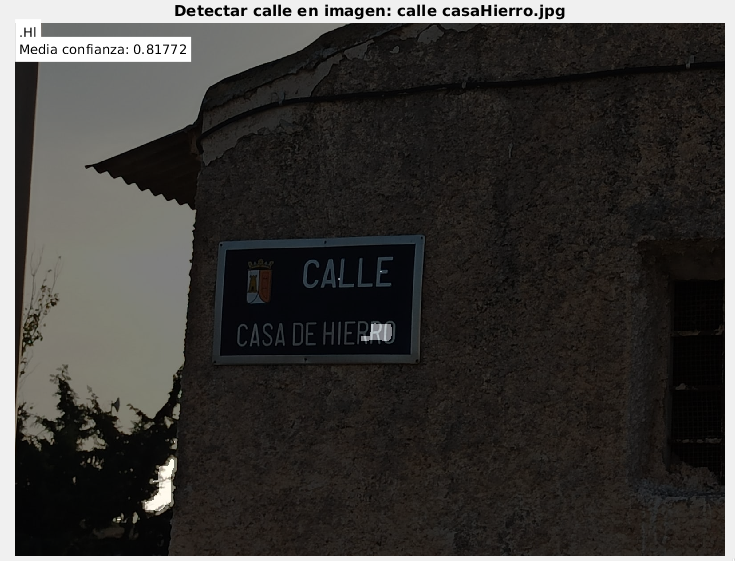
\includegraphics[width=0.65\textwidth]{img/2_10.png}
			\caption{[2] Imagen final Calle Casa de Hierro}
		\end{center}
	\end{figure}
	
	\pagebreak
	
\section{Código desarrollado}
\label{section: codigo}
\noindent En este apartado se encuentra el código integro utilizado para todas las imágenes. Es importante remarcar que todas las imágenes utilizan los mismos elementos estructurantes, por lo que se trata de un algoritmo genérico. Lo único que cambia es la parte de detección de bordes que hemos comentado en el apartado anterior.

\begin{lstlisting}[language=matlab, caption={Código implementado para segmentación y OCR de carteles de calles, utilizando morfología matemática}]
%% Detectar placas de calles
% SRC: https://es.mathworks.com/help/images/detecting-a-cell-using-image-segmentation.html
%clc,
close all

dataset_images = {'calle_condesaPeralta.jpg', ...   %1: OK
	'callejon_soledad_2.jpg', ...     %2: OK
	'calle_aire.jpg', ...             %3: OK
	'calle_sanAgustin.jpg', ...       %4: OK 
	'calle_jabonerias.jpg', ...       %5: OK
	'calle_garciaLorca.jpg', ...      %6: OK
	'calle_juanFernandez.jpg', ...    %7: OK (sale alguna ventana)
	'calle_tolosa.jpg', ...           %8: OK
	'calle_pepeConesa.jpg', ...       %9: OK
	'calle_casaHierro.jpg'};         %10: OK

%j = 5;
for j=1:length(dataset_images) 
	disp([ num2str(j) '. Ejecutando morfologia para la imagen: ' dataset_images{j}])

	% Leer imagen
	img = imread(['./photos/' dataset_images{j}]);
	img_rgb = img;
	img = im2double(rgb2gray(img));
	%figure, imagesc(img), axis off image, colormap gray

	% Detectar bordes (segmentacion)
	[x, thresshold] = edge(img, 'sobel');
	% Valor de ajuste para resaltar todavia mas los bordes de la placa
	k = 1.2;  
	mask = edge(img, 'sobel', thresshold * k);
	%figure, imagesc(mask), axis off image, colormap gray

	% Detecctar bordes (gradiente morfologico)
	% SRC: https://blogs.mathworks.com/steve/2006/09/25/dilation-erosion-and-the-morphological-gradient/
	struc_elemGrad = strel('diamond', 2);
	mask = im2bw(imdilate(img, struc_elemGrad) - imerode(img, struc_elemGrad));
	%figure, imagesc(mask), axis off image, colormap gray, colorbar

	% Dilatar la imagen
	struct_elem90 = strel('line', 12, 90);
	struct_elem0 = strel('line', 12, 0);
	mask_dilate = imdilate(mask, [struct_elem90 struct_elem0]);
	%figure, imagesc(mask_dilate), axis off image, colormap gray

	% Llenar brechas interiores
	mask_fill = imfill(mask_dilate, 'holes');
	%figure, imagesc(mask_fill), axis off image, colormap gray

	% Retirar los objetos no conectados con el borde
	mask_noborder = imclearborder(mask_fill, 4);
	%figure, imagesc(mask_noborder), axis off image, colormap gray,

	% Suavizamos el objeto
	struct_elemD = strel('rectangle', [12 15]);
	mask_final = imerode(mask_noborder, struct_elemD);
	mask_final = imerode(mask_final, struct_elemD);
	%figure, imagesc(mask_final), axis off image, colormap gray

	% Visualizar segmentacion
	% src: https://es.mathworks.com/help/images/ref/imfuse.html
	%img_fuse = imfuse(img, BWfinal, 'falsecolor', 'ColorChannels', [1 2 1]);
	%figure, imagesc(img_fuse), axis off image, colormap gray

	% Multiplicar
	img_mult = immultiply(img, mask_final);
	se_close = strel('line', 3, 90);
	img_mult = imclose(img_mult, se_close);
	%figure, imagesc(img_mult), axis off image, colormap gray

	% OCR
	% SRC: https://es.mathworks.com/help/vision/ref/ocr.html
	% SRC: https://es.mathworks.com/help/vision/ug/recognize-text-using-optical-character-recognition-ocr.html
	% SRC traineddata: https://github.com/tesseract-ocr/tessdata/blob/074c37215b01ab8cc47a0e06ff7356383883d775/spa.traineddata
	results_ocr = ocr(img_mult, 'TextLayout', 'Block', 'Language', {'./tessdata/spa_old_2015.traineddata'});
	%results_ocr = ocr(img_mult, 'TextLayout', 'Block');

	% Obtenemos el texto del OCR
	string_calle = '';
	for i=1:length(results_ocr.Words)
		if i==1
			string_calle = results_ocr.Words{i};
		else
			string_calle = strcat(string_calle, [' ' results_ocr.Words{i}]);
		end
	end
	disp(['El nombre de la calle es: ' string_calle])

	% Overlay imagen original con recuadro 
	% [Falla cuando hay muchos cuadros]
	% SRC: append https://es.mathworks.com/help/vision/ug/recognize-text-using-optical-character-recognition-ocr.html
	%calle_BBox(1) = results_ocr.WordBoundingBoxes(1,1);
	%calle_BBox(2) = results_ocr.WordBoundingBoxes(2,2);
	%calle_BBox(3) = results_ocr.WordBoundingBoxes(1,3);
	%calle_BBox(4) = results_ocr.WordBoundingBoxes(2,4);
	%img_box = insertObjectAnnotation(I, 'rectangle', calle_BBox, string_calle);
	%figure, imagesc(img_box), axis off image, colormap gray

	% Grado de confianza
	grade_confidence = mean(results_ocr.WordConfidences);
	str_confidence = ['Media confianza: ' num2str(grade_confidence)];
	disp(str_confidence);

	% Overlay
	% SRC: https://es.mathworks.com/help/vision/ref/ocr.html
	figure('Position', get(0, 'Screensize')),
	imagesc(imfuse(img_rgb, mask_final, 'blend')),
	axis off image,
	colormap gray,
	title(['Detectar calle en imagen: ' strrep(dataset_images{j},'_',' ')])
	% Nombre de la calle
	text(10, 20, string_calle, 'BackgroundColor', [1 1 1])
	% Confianza
	text(10, 60, str_confidence, 'BackgroundColor', [1 1 1])
	disp('********')
end
\end{lstlisting}

\section{Referencias y bibliografía consultada}
\begin{itemize}
	
	%1
	\item
	\href{https://es.mathworks.com/help/images/detecting-a-cell-using-image-segmentation.html}{Mathworks: Detectar células mediante detección y morfología de bordes}
	
	%2
	\item
	\href{https://blogs.mathworks.com/steve/2006/09/25/dilation-erosion-and-the-morphological-gradient/}{Mathworks: Dilatación, erosión y el gradiente morfológico}
	
	%3
	\item
	\href{https://es.mathworks.com/help/images/ref/imfuse.html}{Mathworks: imfuse}
	
	%4
	\item
	\href{https://es.mathworks.com/help/images/ref/imclearborder.html}{Mathworks: imclearborder}
	
	%5
	\item
	\href{https://es.mathworks.com/help/images/ref/edge.html}{Mathworks: edge}
	
	%6
	\item
	\href{https://es.mathworks.com/help/vision/ug/recognize-text-using-optical-character-recognition-ocr.html}{Mathworks: \textit{Recognize Text Using Optical Character Recognition (OCR)}}
	
	%7
	\item
	\href{https://es.mathworks.com/help/vision/ref/ocr.html}{Mathworks: OCR}
\end{itemize}
	
\end{document}